% Hlavicka pro protokoly z fyzikalniho praktika.
% Verze pro: LaTeX
% Verze hlavicky: 22. 2. 2007
% Autor: Ustav fyziky kondenzovanych latek
% Ke stazeni: www.physics.muni.cz/ufkl/Vyuka/
% Licence: volne k pouziti, nejlepe k vcasnemu odevzdani protokolu z Vaseho mereni.


\documentclass[czech,11pt,a4paper]{article}
\usepackage[T1]{fontenc}
\usepackage{graphicx, animate}
\usepackage{mathtools}
\usepackage{amssymb}
\usepackage{amsthm}
\usepackage{thmtools}
\usepackage{xcolor}
\usepackage{nameref}
\usepackage{babel}
\usepackage{hyperref}
\usepackage{multicol}
\usepackage[export]{adjustbox}
\usepackage{subcaption}
\usepackage{caption}
\usepackage{multirow}
\usepackage{float}
\usepackage{placeins}

\graphicspath{ {./images/} }
\usepackage[backend=biber,style=numeric]{biblatex}       % [1], [2], ...




\addbibresource{ref.bib}


%%% Nemente:
\usepackage[margin=2cm]{geometry}
\newtoks\jmenopraktika \newtoks\jmeno \newtoks\datum
\newtoks\obor \newtoks\skupina \newtoks\rocnik \newtoks\semestr
\newtoks\cisloulohy \newtoks\jmenoulohy

%%% Nemente - konec.


%%%%%%%%%%% Doplnte pozadovane polozky:

\jmenopraktika={Fyzikální praktikum 3}  % nahradte jmenem vaseho predmetu
\jmeno={Teodor Duraković}            % nahradte jmenem mericiho
\datum={25.~února 2024}        % nahradte datem mereni ulohy
\obor={F}                     % nahradte zkratkou vami studovaneho oboru
\skupina={Út 14:00}            % nahradte dobou vyuky vasi seminarni skupiny
\rocnik={II}                  % nahradte rocnikem, ve kterem studujete
\semestr={IV}                 % nahradte semestrem, ve kterem studujete

\cisloulohy={3}               % nahradte cislem merene ulohy
\jmenoulohy={Milikanův experiment}           % nahradte vlhkosti vzduchu pri mereni (v %)

%%%%%%%%%%% Konec pozadovanych polozek.


%%%%%%%%%%% Uzitecne balicky:

%%%%%% Zamezeni parchantu:
\widowpenalty 10000 \clubpenalty 10000 \displaywidowpenalty 10000
%%%%%% Parametry pro moznost vsazeni vetsiho poctu obrazku na stranku
\setcounter{topnumber}{3}	  % max. pocet floatu nahore (specifikace t)
\setcounter{bottomnumber}{3}	  % max. pocet floatu dole (specifikace b)
\setcounter{totalnumber}{6}	  % max. pocet floatu na strance celkem
\renewcommand\topfraction{0.9}	  % max podil stranky pro floaty nahore
\renewcommand\bottomfraction{0.9} % max podil stranky pro floaty dole
\renewcommand\textfraction{0.1}	  % min podil stranky, ktery musi obsahovat text
\intextsep=8mm \textfloatsep=8mm  %\intextsep pro ulozeni [h] floatu a \textfloatsep pro [b] or [t]

% Tecky za cisly sekci:
\renewcommand{\thesection}{\arabic{section}.}
\renewcommand{\thesubsection}{\thesection\arabic{subsection}.}
\renewcommand{\thesubsubsection}{\thesubsection\arabic{subsubsection}.}
% Jednopismenna mezera mezi cislem a nazvem kapitoly:
\makeatletter \def\@seccntformat#1{\csname the#1\endcsname\hspace{1ex}} \makeatother


%%%%%%%%%%%%%%%%%%%%%%%%%%%%%%%%%%%%%%%%%%%%%%%%%%%%%%%%%%%%%%%%%%%%%%%%%%%%%%%
%%%%%%%%%%%%%%%%%%%%%%%%%%%%%%%%%%%%%%%%%%%%%%%%%%%%%%%%%%%%%%%%%%%%%%%%%%%%%%%
% Zacatek dokumentu
%%%%%%%%%%%%%%%%%%%%%%%%%%%%%%%%%%%%%%%%%%%%%%%%%%%%%%%%%%%%%%%%%%%%%%%%%%%%%%%
%%%%%%%%%%%%%%%%%%%%%%%%%%%%%%%%%%%%%%%%%%%%%%%%%%%%%%%%%%%%%%%%%%%%%%%%%%%%%%%

\begin{document}
	
	%%%%%%%%%%%%%%%%%%%%%%%%%%%%%%%%%%%%%%%%%%%%%%%%%%%%%%%%%%%%%%%%%%%%%%%%%%%%%%%
	% Nemente:
	%%%%%%%%%%%%%%%%%%%%%%%%%%%%%%%%%%%%%%%%%%%%%%%%%%%%%%%%%%%%%%%%%%%%%%%%%%%%%%%
	\thispagestyle{empty}
	
	{
		\begin{center}
			\sf 
			{\Large Ústav fyziky a technologií plazmatu Přírodovědecké fakulty Masarykovy univerzity} \\
			\bigskip
			{\huge \bfseries FYZIKÁLNÍ PRAKTIKUM} \\
			\bigskip
			{\Large \the\jmenopraktika}
		\end{center}
		
		\bigskip
		
		\sf
		\noindent
		\setlength{\arrayrulewidth}{1pt}
		\begin{tabular*}{\textwidth}{@{\extracolsep{\fill}} l l}
			\large {\bfseries Zpracoval:}  \the\jmeno & \large  {\bfseries Naměřeno:} \the\datum\\[2mm]
			\large  {\bfseries Obor:} \the\obor  \hspace{40mm}  {\bfseries Skupina:} \the\skupina %
			%{\bfseries Ročník:} \the\rocnik \hspace{5mm} {\bfseries Semestr:} \the\semestr  
			&\large {\bfseries Testováno:}\\
			\\
			\hline
		\end{tabular*}
	}
	
	\bigskip
	
	{
		\sf
		\noindent \begin{tabular}{p{3cm} p{0.6\textwidth}}
			\Large  Úloha č. {\bfseries \the\cisloulohy:} \par
			\smallskip
			&\Large \bfseries \the\jmenoulohy  \\[2mm]
		\end{tabular}
	}
	
	\vskip1cm
	
	%%%%%%%%%%%%%%%%%%%%%%%%%%%%%%%%%%%%%%%%%%%%%%%%%%%%%%%%%%%%%%%%%%%%%%%%%%%%%%%
	% konec Nemente.
	%%%%%%%%%%%%%%%%%%%%%%%%%%%%%%%%%%%%%%%%%%%%%%%%%%%%%%%%%%%%%%%%%%%%%%%%%%%%%%%
	
	%%%%%%%%%%%%%%%%%%%%%%%%%%%%%%%%%%%%%%%%%%%%%%%%%%%%%%%%%%%%%%%%%%%%%%%%%%%%%%%
	%%%%%%%%%%%%%%%%%%%%%%%%%%%%%%%%%%%%%%%%%%%%%%%%%%%%%%%%%%%%%%%%%%%%%%%%%%%%%%%
	% Zacatek textu vlastniho protokolu
	%%%%%%%%%%%%%%%%%%%%%%%%%%%%%%%%%%%%%%%%%%%%%%%%%%%%%%%%%%%%%%%%%%%%%%%%%%%%%%%
	%%%%%%%%%%%%%%%%%%%%%%%%%%%%%%%%%%%%%%%%%%%%%%%%%%%%%%%%%%%%%%%%%%%%%%%%%%%%%%%
	
	\begin{multicols}{2}
		\section{Zadání}
	
Změřte velikost elementárního náboje pomocí rychlostí padající a stoupající olejové kapičky
v homogenním elektrickém poli. Proveďte měření rychlostí alespoň padesáti kapek. Výsledek
srovnejte s tabulkovou hodnotou.\\

		\section{Teorie}
		
		Milikanův experiment pomocí sledování pohybu nabité kapičky v poli dokáže určit velikost elementárního náboje. V naší realizaci experimentu vstřikujeme kapičky do komory s kondenzátorem, přičemž se některé kapky dokáží nabíjet třením i působením radioaktivního zdroje $\alpha$-částic. Napětí na kondenzátoru lze měnit, stejně jako jeho polaritu.
		
		Na kapičku v experimentu působí tíhová síla (1), vztlaková síla (2), proti směru pohybu třecí síla (3) a směrem k anodě síla elektrická (4).
		\begin{align}
			F_{g}&=\frac{4}{3} \pi r^{3} \rho g,\\
			F_{t}&=6 \pi \eta r v,\\
			F_{e}&=|q| E \text {, }
		\end{align}
		Kombinací těchto rovnic získáme vztah pro poloměr kapky a pro náboj kapky:
		\begin{align}
			r&=\sqrt{\frac{9 \eta\left(v_{1}-v_{2}\right)}{4 g\left(\rho-\rho_{v z}\right)} }\\
			|q|&=3 \pi \eta r \frac{v_{1}+v_{2}}{E} .			
		\end{align}
		
		\section{Zpracování dat}
		V rámci experimentu zaznamenáváme obraz, který je následně potřeba zpracovat tak, abychom dostali (co nejjednodušším způsobem) co nejvíce validních rychlostí. Pracujeme s přiloženým programem [1] - u něj sledujeme, že nejlépe zpracovává zhruba dvousekundové sekvence. Proto všechen získaný materiál (circa 40 minut čistého videa) stříháme na dvousekundové překrývající se sekvence. Dvousekundový interval je ideální i proto, že program při naší frekvenci převracení polarity v daném intervalu nalezne maximálně jedinou instanci změny polarity a zároveň nám dva po sobě jdoucí intervaly netvoří duplikáty.	Takto zpracovaná data následně manuálně filtrujeme; využíváme obrazového výstupu programu, přičemž vidíme závislosti měřených poloh na čase (resp. obrazových souřadnicích) i provedené fity, jejichž výstupem jsou rychlosti. Tento proces je blíže znázorněn na obr. 1.
		\begin{figure}[H]
			\centering
			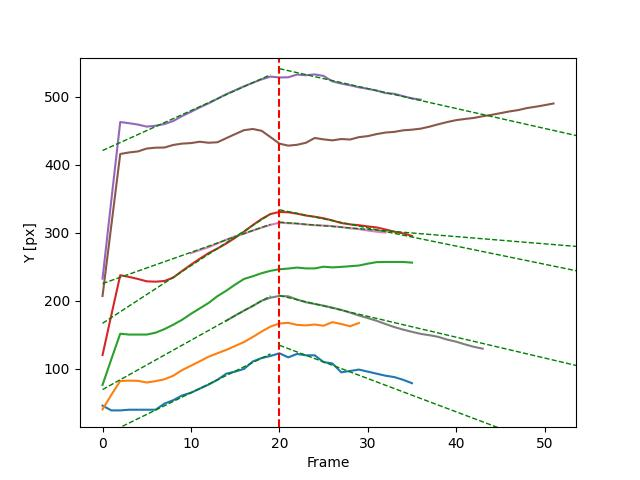
\includegraphics[width=0.8\linewidth]{segment_44.mp4_plot}
			\caption{{\small Výstup programu s provedenými fity - v tomto případě odstraňujeme výsledky pro fit fialové a modré křivky}}
			\label{fig:segment44}
		\end{figure}
		Tímto způsobem získáváme rychlosti pro různé hodnoty kondenzátorového napětí. 
		\subsection{Množství získaných dat}
		Místo požadovaných padesáti hodnot pracujeme se zhruba šesti sty - zejména proto, že chyby v rámci měření nelze zanedbat a takto předpokládáme, že se nám budou tvořit lépe viditelné clustery nábojů kolem skutečných hodnot - celočíselných násobků elementárního náboje. Naprosto ideální by bylo se dostat na vyšší počty hodnot, pak by velikost elementárního náboje bylo možno určit jednoduše z pouhé vizuální analýzy histogramu. 
		
		Z dat získaných výše uvedeným popisem pomocí formule (5), (6) získáme hodnoty poloměrů kapek i nábojů. Z porovnání dat se skutečnou hodnotou elementárního náboje $e$ lze získat rozdělení konkrétních hodnot náboje (resp. celočíselných násobků $e$), tato data lze pomocí Monte Carlo simulace využít pro predikci výsledků při větším, resp. menším počtu dat.
		
		Obr. 2, 3 ukazují skutečné rozdělení hodnot a rozdělení získané z popsané simulace:
		\begin{figure}[H]
			\centering
			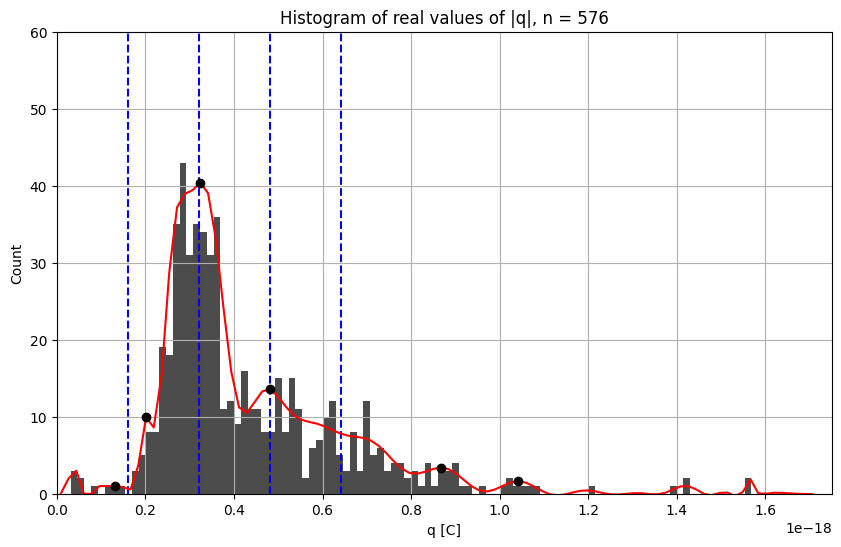
\includegraphics[width=0.8\linewidth]{histogramreal}
			\caption{Skutečný histogram získaný z měřených dat, vertikální čáry označují celočíselné násobky $e$, $n <5$, histogram je zároveň vyhlazen ve funkci, následně jsou nalezena lokální maxima.}
			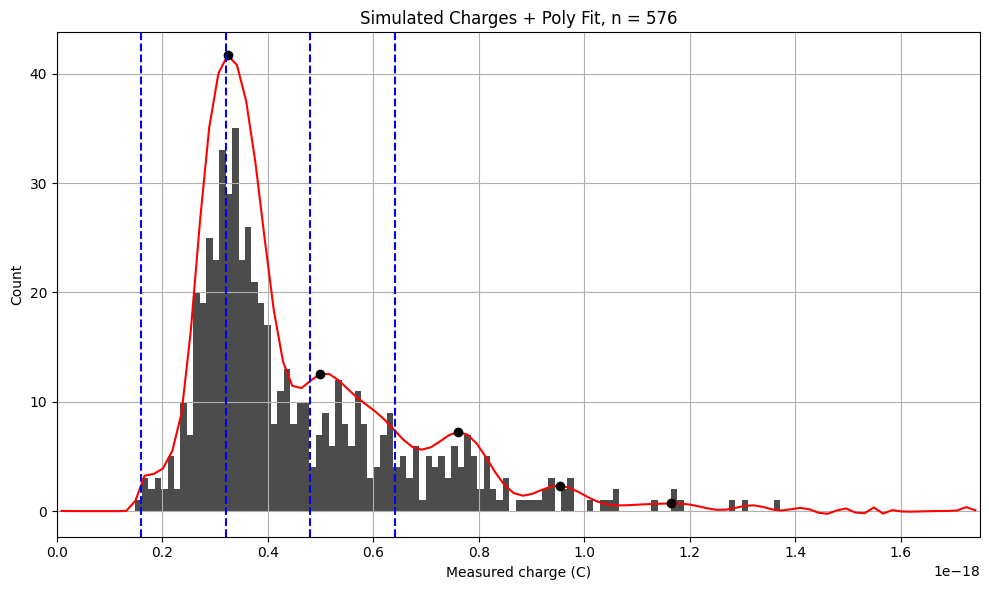
\includegraphics[width=0.8\linewidth]{histogramMC1}
			\caption{diagram MC simulace se stejným počtem nábojů}
		\end{figure}
		 Lze pozorovat, že při menším počtu vzorků (požadovaných padesáti) je rozlišení, a tím i samotná přesnost odhadu mnohem nižší (obr. 4), stejně tak lze najít počet vzorků, ze kterého je velikost elementárního náboje jasně viditelná. Kvůli rozdělení nábojů - maxima pro $n=2$ a mnohem nižší četnosti ostatních nábojů bychom jasná tři lokální maxima získali až při zhruba deset až stokrát větším vzorku (extrémní případ - vzorek o velikosti 1 000 000 je na obr. 5).
		 
		 \begin{figure}[H]
		 	\centering
		 	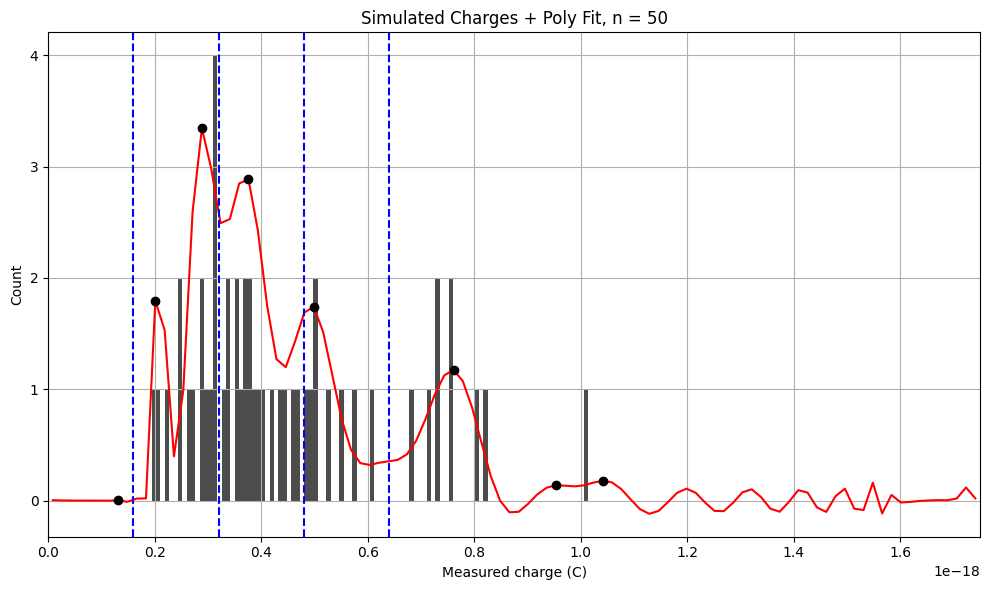
\includegraphics[width=0.8\linewidth]{histogamMC4}
		 	\caption{MC simulace se vzorkem n = 50}
		 	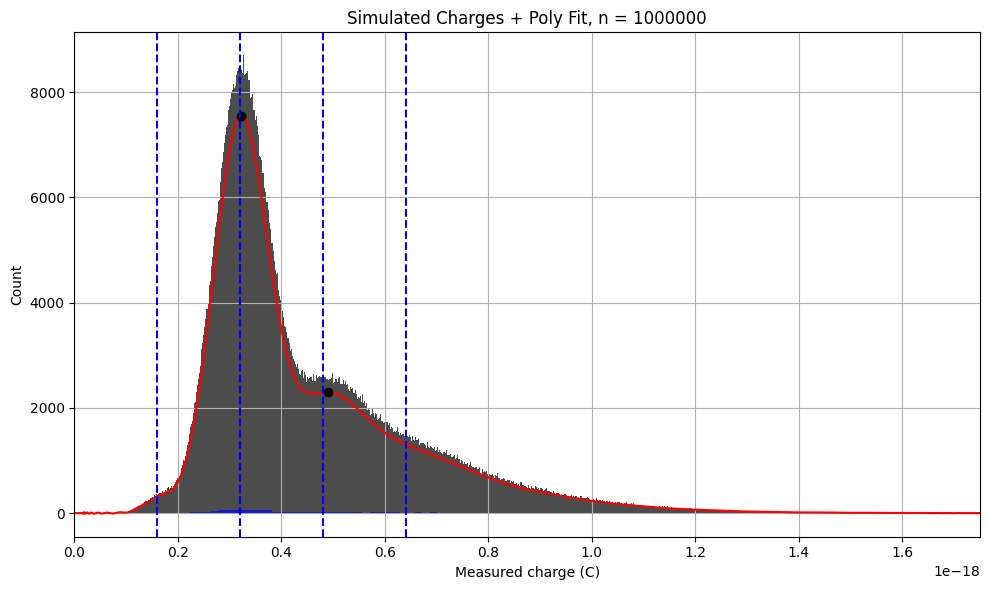
\includegraphics[width=0.8\linewidth]{histogramMC5}
		 	\caption{MC simulace se vzorkem n = 1 000 000}

		 \end{figure}
		 \section{Možnosti výpočtu hodnoty elementárního náboje}
		 Hodnotu elementárního náboje lze získat vícero možnými způsoby - buď s využitím znalosti skutečné hodnoty, nebo bez něj. Pracujeme-li se skutečnou hodnotou, lze využít samotného histogramu - pozorujeme totiž, že maximální zastoupení hodnot blízkých $q = 2e$ i v samotné vyhlazené funkci realizuje globální maximum právě v bodě $q = 2e$ - takovému výsledku se nelze divit, přeci jen vyhlazení (v tomto případě polynomický fit velmi vysokého řádu (2500)) není nic jiného než přiblížení výsledkům většího vzorku. Lze tedy využít získaných lokálních maxim v $q_2 \approx 2e $ a $q_3 \approx 3e$:
		 {\small \begin{align*}
		 	q_2 = 3.2\pm 0.3\cdot10^{-19} &\quad q_3 = 4.8\pm 0.3\cdot 10^{-19} \,\mathrm{C} \\
		 	&\quad e = 1.61\pm 0.08 \cdot 10^{-19} \,\mathrm{C}
		 \end{align*}}
	 	Alternativně lze pro všechny naměřené náboje určit, kterému z celočíselných násobků elementárního náboje příslušejí (tj. ke kterému násobku jsou nejblíže). Jak lze však vidět na obr. 2, kvůli velkým odchylkám je četnost nábojů s hodnotami mimo celočíselný násobek elementárního náboje nezanedbatelná. Řád tedy získáme formulí $n = \mathrm{round}(\frac{q}{e})$, následně lze vykreslit závislost náboje na řádu. Ze směrnice lineárního fitu získáme hodnotu elementárního náboje (obr. 6):
		 \begin{figure}[H]
	 	 	\centering
	 	 	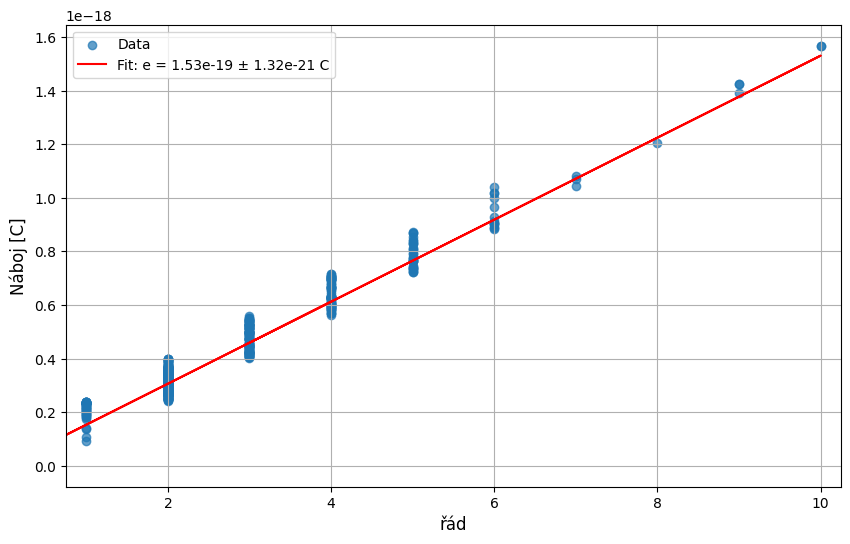
\includegraphics[width=0.8\linewidth]{fit1}
	 	 	\caption{Závislost velikosti náboje na řádu}
	 	 	
		 \end{figure}
		 V tomto případě ovšem pouze provádíme jednu operaci (počítáme násobek) a následně postupujeme obráceně - jde o řešení přinejmenším polovičaté - při takovém zjednodušení by rovnou bylo možno filtrovat hodnoty $q$, aby ze vzorku byly vyřazeno vše s větší odchylkou - v takové situaci bychom získávali ještě lepší výsledek, jak lze pozorovat na obr. 7:
		 
		 \begin{figure}[H]
		 	\centering
		 	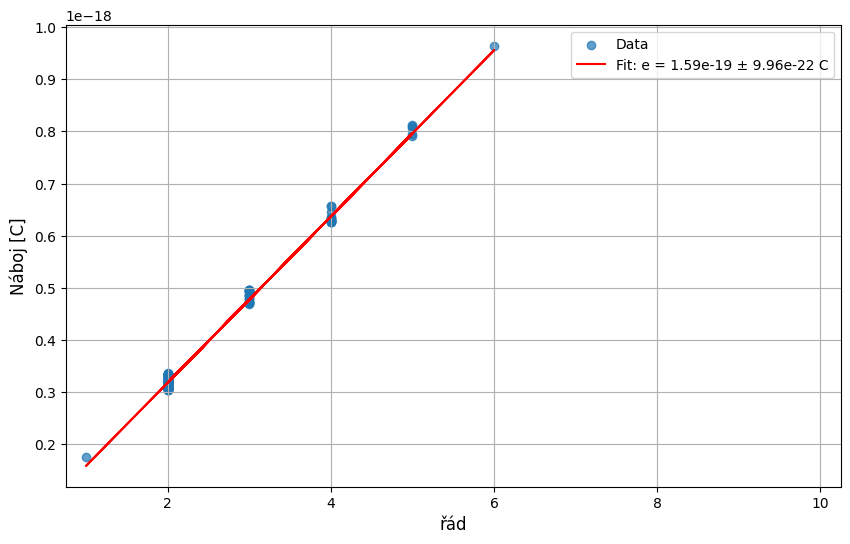
\includegraphics[width=0.8\linewidth]{fit2}
		 	\caption{Závislost velikosti náboje na řádu, odstraněny jsou všechna data, jejichž n se před zaokrouhlením od celého čísla liší o více než 0.1}
		 	
		 \end{figure}
		 
		 Lepší způsob nalezení hodnoty $e$ je tuto hodnotu odhadnout.
		 \subsection{Odhad hodnoty elementárního náboje - minimalizace chybové funkce}
		 V této metodě zpracování dat již nevyužíváme přesnou hodnotu $e$. Místo toho vycházíme z předpokladu, že veškeré hodnoty měřených nábojů splňují $q_i \approx n_i \cdot e ,\,\ n_i \in \mathbb{N}$. Pro arbitrární hodnotu $e$ lze pro každé $q_i$ určit řád násobku $n_i = \mathrm{round}(\frac{q_i}{e})$, s těmito údaji lze získat aproximovaný náboj \\ $\hat{q}_i = n_i \cdot e$. Chybovou funkci $S(e) = \sum_i (q_i - \hat{q}_i)^2$ (rozdíl kvadrátů hodnot nábojů) chceme minimalizovat - nalézt takovou hodnotu $e$, pro kterou jsou odchylky nejmenší. Celý problém se tedy redukuje na poměrně jednoduchou optimalizační úlohu. Zde se však setkáváme se značnou asymetrií funkce $S(e)$, čímž je hledání minima mnohem složitější (Obr. 8). 
			
		\begin{figure}[H]
			\centering
			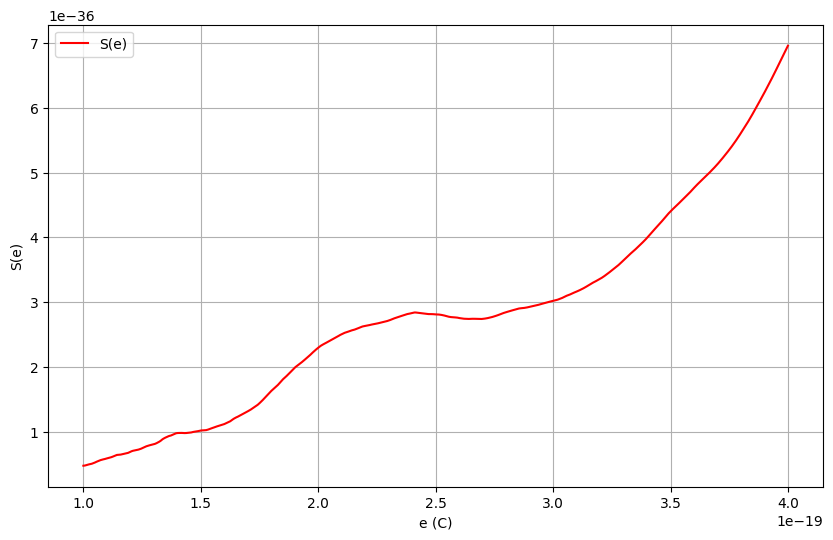
\includegraphics[width=0.5\linewidth]{plot3}
			\caption{Průběh chybové funkce $S(e)$}
			
		\end{figure}	 
		Ze samotného histogramu i hodnot náboje lze $(1,4)\cdot 10^{-19}$ vyvodit jako poměrně rozumný interval, zároveň víme, že skutečná hodnota $e$ se musí ukrývat při nižších hodnotách měřeného náboje. Asymetrii chybové funkce se rozhodujeme vyřešit odstraněním monotónnosti. Provádíme krok, který může být brán jako přinejmenším kontroverzní: odstraňujeme směrnici funkce (konkrétně funkci nejdřív lineárně fitujeme), následně hodnoty $S(e)$ upravujeme právě získanou směrnicí na $S_2(e) = S(e) - (k*e)$. Tento krok by neměl zásadně ovlivnit lokální minimum a další postup zjednodušuje na pouhé hledání tohoto minima. Tímto postupem získáváme výsledky (Obr.9):
		
		\begin{figure}[H]
			\centering
			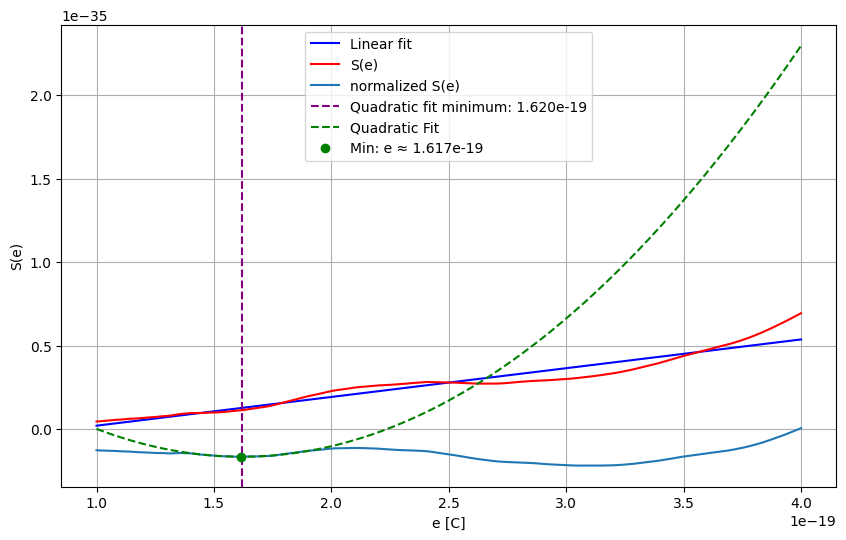
\includegraphics[width=0.8\linewidth]{fit4}
			\caption{Chybová funkce $S(e)$, její lineární fit (tmavě modrá), normovaná chybová funkce $S(e)$, (světle modrá), kvadratický fit první oblasti s lokálním minimem (zelená-čárkovaná) a hodnota lokálního minima (fialová a žlutá čárkovaná)}
			
		\end{figure}	 
			 
			 Jako výsledek získáváme:
			 \begin{equation*}
			 	e = 1.617 \pm 0.15 \cdot 10^{-19} \,\mathrm{C} 
			 \end{equation*}
			 
	 	Tento postup lze ověřit i na simulovaných datech; Na obr. 10 pozorujeme, že je průběh pro $n = 100 000$ v podstatě identický, pouze vyhlazenější.
	 	
	 	\begin{figure}[H]
	 		\centering
	 		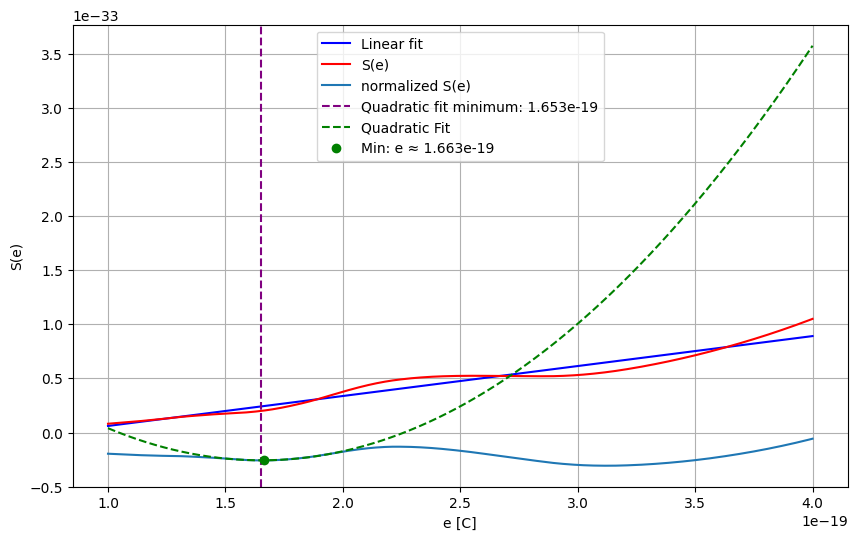
\includegraphics[width=0.8\linewidth]{fit5}
	 		\caption{Vizualizace z obr. 9 zpracovávající data z MC simulace pro n = 100 000}
	 		
	 	\end{figure}
	 	Naopak odstraníme-li šum, ať již z reálných nebo vygenerovaných hodnot, tento způsob zpracování nám skutečně bude dávat hodnotu bližší e, zároveň budeme pozorovat viditelný pokles směrnice:
	 	
	 	\begin{figure}[H]
	 		\centering
			\animategraphics[autoplay, loop, width=1\linewidth]{4}{gif}{1}{6}

	 		\caption{Animace zpracování dat s postupně menšími odchylkami od $n*e$ (původní odchylka-0.6násobek původní odchylky). Lze pozorovat viditelný pokles směrnice (\textit{K správnému zobrazení animace je nutno dokument otevřít v programu, který animace podporuje (kupř. Adobe Acrobat)}}
	 		
	 	\end{figure}
	 	\subsection{Histogram aproximovaných elementárních nábojů}
	 	Můžeme též využít zmíněné řády násobků $n_i$ a vykreslit četnosti aproximovaných nábojů $\hat{e} = \frac{q_i}{n_i}$. Zde můžeme očekávat normální rozdělení četností. Získáváme (obr. 12):
	 	\begin{figure}[H]
	 		\centering
	 		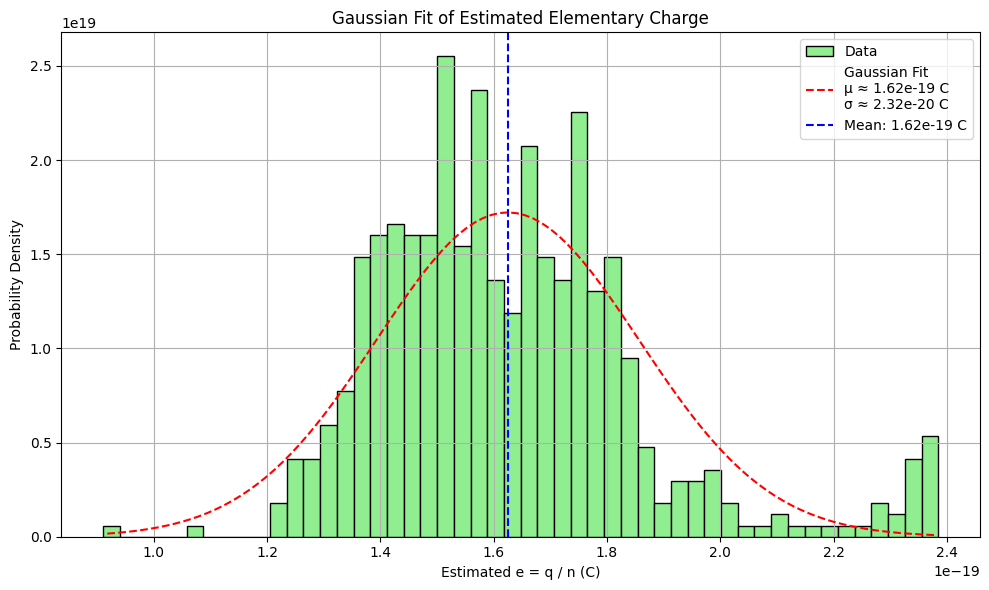
\includegraphics[width=0.8\linewidth]{gauss1}
	 		\caption{Histogram aproximovaných elementárních nábojů}
	 		
	 	\end{figure}
	 	\begin{equation*}
	 		e = 1.62 \pm 0.2 \cdot 10^{-19} \, \mathrm{C}
	 	\end{equation*}
	 	Znovu lze smysl této metody ověřit na větším, simulovaném vzorku, jak lze pozorovat na obr. 13. Stejných, byť vizuálně mnohem méně působivých, výsledků dosahujeme i "očištěním" skutečných dat způsobem jak na Obr. 7. 
	 	\begin{figure}[H]
	 		\centering
	 		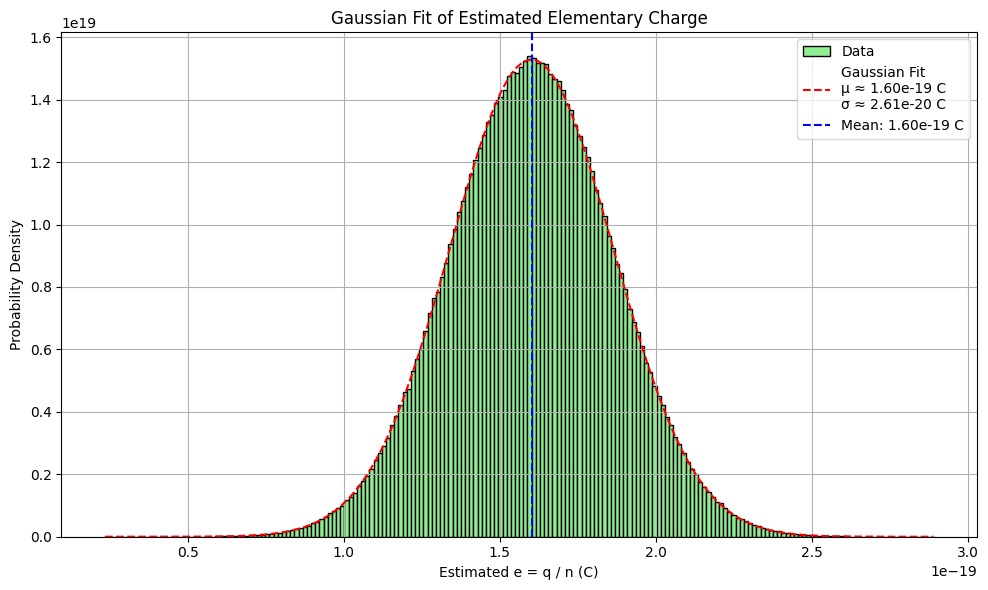
\includegraphics[width=0.8\linewidth]{gauss2}
	 		\caption{Histogram aproximovaných elementárních nábojů, pro velikost vzorku $n = 1\, 000\,000 $}
	 		
	 	\end{figure}
		
		
		\section{Závěr}
		Úspěšně se nám podařilo replikovat Milikanův experiment a získaná data zpracovat. Jako nejúspěšnější vyhodnocujeme metodu analýzy histogramu, po ní metodu histogramu aproximovaných elementárních nábojů a metodu získání hodnoty $e$ prostřednictvím minimalizace chybové funkce. Získali jsme ke skutečné hodnotě $e = 1.602176 \cdot 10^{-19}\,\mathrm{C}$\cite{NIST} výsledky poměrně blízké, získali jsme jmenovitě hodnoty $e_1 = 1.61\pm 0.08 \cdot 10^{-19}, e_2 = 1.62\pm 0.2 \cdot 10^{-19}, e_3 = 1.62 \pm 0.15 \cdot 10^{-19} \,\mathrm{C}  $
		
\printbibliography

			\end{multicols}
		
		
		% Nakonec nezapomeňte projet text programem vlna nebo vlnka, např.
		% 	vlna -m -l -n mojeuloha.tex
		% nebo zkontrolovat a opravit jednopísmenné předložky na koncích řádků ručně.

\end{document}
